%%%%%%%%%%%%%%%%%%%%%%%%%%%%%%%%%%%%%%%%%%%
%   Simple and elegant academic report    %
%   Copyright by Artur M. Brodzki, 2019   %
%%%%%%%%%%%%%%%%%%%%%%%%%%%%%%%%%%%%%%%%%%%

\documentclass{eiti-raport}

\usepackage[
	english,
	polish
]{babel}
\usepackage{polski}

%------------------------------------------

\begin{document}

\author{Artur M. Brodzki}
\date{\today}
\subject{Nazwa przedmiotu}
\title{Tytuł raportu}

\pagenumbering{arabic}
\maketitle

%------------------------------------------
% MAIN CONTENTS
%------------------------------------------

\begin{multicols}{2}

\section{Wstęp} \label{sec:intro}
\lipsum[1-2]

\section{Rozdział 2} \label{sec:2}
\lipsum[3]
\begin{center}
	\label{fig:anzelm}
	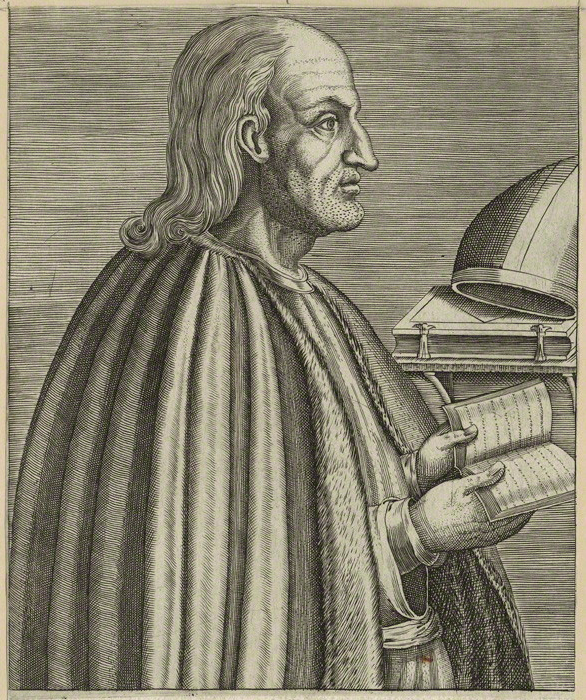
\includegraphics[width=0.5\linewidth]{img/anzelm.PNG}
	\captionof{figure}{Anzelm z Canterbury.}
\end{center}
\lipsum[4]
\begin{align*}
E & = m c^2 \\ 
y & = a x^2 + bx + c
\end{align*}
\lipsum[5]

\section{Podsumowanie} \label{sec:summary}
\lipsum[6]

\section*{Literaura}

\noindent [Anderson, 1990] Anderson, C. A. (1990). Some emendations of G\"odel’s ontological proof. \textit{Faith and Philosophy}, str. 291–303. Dostęp zdalny (PDF): \url{https://somewebsite.com/ontological-proof22.pdf}  
\\ \\
\noindent [Anderson, 1996] Anderson, C. A.; Geettings, M. (1996). G\"odel’s ontological proof revisited. \textit{Lecture Notes in Logic}, str. 167–172. Dostęp zdalny (PDF): \url{https://projecteuclid.org/download/pdf_1/euclid.lnl/1235417020}


\end{multicols}
\end{document}
